\section{Introduction}

Training data processing---assembly, subword tokenization, sequence packing (concatenating records into fixed-length training chunks)---destroys the mapping between individual records and their original contributors. Trainers cannot locate specific data for removal requests, license audits, or quality tracing; the only recourse is file-level over-deletion (discarding entire files when only individual records need removal).

Existing tools address different parts of this gap (Table~\ref{tab:provenance-comparison}). Data versioning systems (DVC, LakeFS, Delta Lake) and experiment trackers (MLflow, Weights \& Biases [W\&B]) operate at file or dataset granularity. Provenance frameworks (yProv4ML, DLProv) capture pipeline lineage but not per-record authorship; Chen et al.~\cite{chen2026finegrained} propose fine-grained traceability with contribution scores but focus on training-stage data usage auditing rather than authorship attribution. Dolt~\cite{dolt} versions database rows but lacks contributor-level attribution and revocation; WikiWho~\cite{flock2014wikiwho} provides token-level attribution on Wikipedia but no revocation. ForSId~\cite{dangelo2025forsid} infers forget sets post-hoc but requires a trained model, and ERASURE~\cite{dangelo2025erasure} benchmarks unlearning evaluation but does not construct forget sets from provenance. None provide record-level author attribution with deterministic queries, license tracking, and no model access.

\begin{table}[t]
	\centering
	\small
	\caption{Provenance tools comparison. Existing systems operate at file, dataset, or experiment granularity; none support record-level author revocation or license tracking.}
	\label{tab:provenance-comparison}
	\setlength{\tabcolsep}{3pt}
	\begin{tabular}{@{}lcccc@{}}
		\toprule
		System & Granularity & Revocation & License & Adoption \\
		\midrule
		DVC~\cite{dvc} & File/dataset & \ding{55} & \ding{55} & 15k+ \\
		LakeFS~\cite{lakefs} & Dataset/table & \ding{55} & \ding{55} & 5k+ \\
		Delta Lake~\cite{deltalake} & Table & \ding{55} & \ding{55} & 8k+ \\
		MLflow~\cite{mlflow} & Experiment & \ding{55} & \ding{55} & Active \\
		W\&B~\cite{wandb} & Experiment & \ding{55} & \ding{55} & Active \\
		yProv4ML~\cite{padovani2025yprov4ml} & Dataset & \ding{55} & \ding{55} & Low \\
		DLProv~\cite{pina2025dlprov} & Task & \ding{55} & \ding{55} & Low \\
		Dolt~\cite{dolt} & Row (version) & \ding{55} & \ding{55} & 23k+\rlap{\footnotemark} \\
		WikiWho~\cite{flock2014wikiwho} & Token & \ding{55} & \ding{55} & Acad. \\
		\rowcolor{blue!10}\textbf{OriginBlame} & \textbf{Rec.+Tok.} & \textbf{\ding{51}} & \textbf{\ding{51}} & \textbf{---} \\
		\bottomrule
	\end{tabular}
\end{table}
\footnotetext{Adoption counts: GitHub stars as of 2026-06. ``Active'' = widely used in industry. ``Acad.'' = academic tool.}

This demonstration presents OriginBlame (\texttt{ob}), a three-layer content-addressable provenance system that propagates author identity through data processing pipelines. \textbf{Key innovations}: (1)~deterministic SHA-256-based provenance requiring no GPU or model access; (2)~record- and token-level attribution that reduces file-level over-deletion to near-parity; (3)~because unlearning algorithms require precise forget sets as input, ob's record-level provenance provides the first deterministic method to construct them---validated with NPO (Negative Preference Optimization)~\cite{zhang2024npo} and RMU (Reliable Machine Unlearning)~\cite{li2024wmdp} on a 1.7B model. The live web application provides eight indexed datasets spanning three domains (Wikipedia, kernel source, and ChatML training data), enabling real-time provenance queries, three-level revocation, and cross-domain comparison.

\begin{figure}[t]
	\centering
	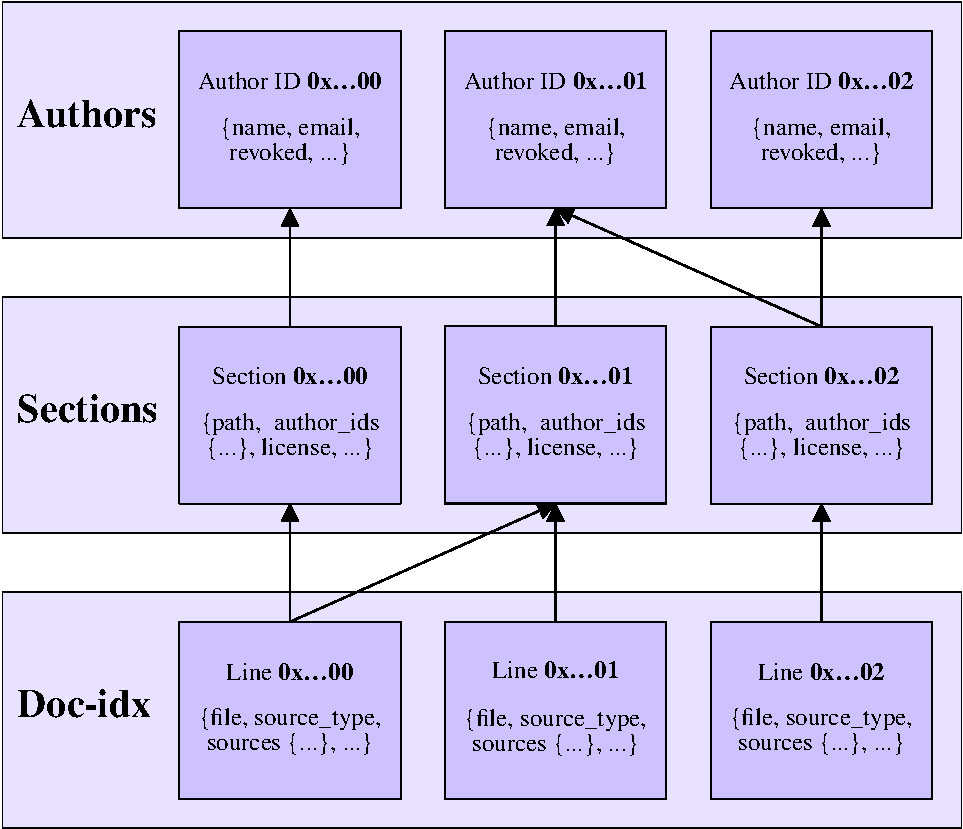
\includegraphics[width=\columnwidth]{figures-cikm/fig2}
	\Description{Three-layer architecture diagram showing Authors, Sections, and Document-Index layers with hash-based sharding.}
	\caption{Three-layer reference architecture with hash-based 256-bucket sharding.}
	\label{fig:three-layer}
\end{figure}
